% !Mode:: "TeX:UTF-8"
\documentclass{xcumcmart}
\usepackage{setspace}
\usepackage{enumerate}
\usepackage{tabu}
% \title{text}这里是显示在第三页的文章标题
\title{基于线性模型的钢水“脱氧合金化”方案优化}
\linespread{1.2} %行距
\begin{document}
\renewcommand\arraystretch{2}

\maketitle
\begin{cnabstract}%此处没有采用sbstract命名,是为了将来如果要加入英文摘要时扩展的方便
\setlength{\parskip}{1.4em} %段落距离

\par \textit{占位文字,待替换题目需要我们通过对合金钢的生产历史数据进行分析,应该利用统计学知识以及数据处理的方法,对数据进行适当的预处理,再根据题目的具体要求,利用合理的指标和算法进行建模,并进行模型检验。}
\par \textbf{关键词:脱氧合金化 回归拟合 线性优化}
\end{cnabstract}

\setlength{\parskip}{1.4em}

%\tableofcontents\newpage%增加目录,要不要都可以。不想要的话,就在本行前加“%”(英文的百分号)
\section{问题重述}
\par 目前,各大钢铁企业为提高竞争力所要解决的重要问题是:如何在保证钢水质量的同时最大限度降低合金钢的生产成本。这要求我们通过历史数据对脱氧合金化环节建立数学模型,在线预测并优化投入合金的种类及数量,最终实现成本-收益最大化目标。我们需要通过题目所给数据解决如下问题:
\begin{enumerate}[(a)]%(\arabic{section}.1)
\setlength{\itemindent}{2em}    %标签缩进量
\item 计算C、Mn两种元素的历史收得率,并分析影响其收得率的主要因素。
\item 基于问题1,对C、Mn元素收得率进行预测,并对模型进行改进。
\item 基于问题2实现钢水脱氧合金化的成本优化计算,并给出合金配料方案。
\item 根据研究结果给炼钢厂提出建议。
\end{enumerate}

\section{问题分析}
\par 题目需要我们通过对合金钢的生产历史数据进行分析,应该利用统计学知识以及数据处理的方法,对数据进行适当的预处理,再根据题目的具体要求,利用合理的指标和算法进行建模,并进行模型检验。
\par 问题一要求我们根据历史数据测算出C、Mn两种元素的历史收得率。计算之前应对数据的缺失情况进行分析,并合理地进行缺失值按行或按列丢弃、均值替代等操作,保证计算的可靠性。针对收得率影响因素的研究,首先使用相关系数进行定性的初步判定,其次增加线性回归进行定量分析。
\par 问题二要求我们对收得率进行预测,并改进模型及算法提高预测的准确性。第一题线性模型可以实现对元素收得率的预测,在此基础上模型改进有以下两点:第一,进一步确定元素收得率在实际工业应用中的可能影响因素,考虑数据缺失情况以及预测模型的需要,处理缺失值较多的变量时,将转炉终点缺失值替换为均值,重新计算收得率;第二,使用多种回归算法,通过合理的回归评价指标确定最佳模型算法。
\par 问题三是目标函数最优化问题,利用第二问的预测模型稍加修改,可实现对连铸合金的元素含量预测,根据题目所给HRB400B型号合金钢的元素含量标准建立线性约束,由于仅需要优化配料的成本,将未知的转炉终点元素含量以及转炉终点温度、钢水质量等无关变量全部使用均值替代,最终建立价格目标函数求解满足条件的最优方案。
\par 问题四则为基于上述问题的分析结果提出本团队的生产建议。

\section{假设与符号}
\subsection{假设条件}
\subsection{符号说明}
\begin{table}[htbp]
	\centering
	\begin{tabu}{l l}
		\tabucline[1.5pt]{-}
		符号 & 说明\\
		\tabucline[1.5pt]{-}
		$\mu$ & 某组数据的平均值\\
		$\sigma$ & 某组数据的标准差\\
		\tabucline[1.5pt]{-}
	\end{tabu}
	\caption{Mn收得率与主要影响因素的相关系数\label{tb:tbs2}}
\end{table}
\section{模型的建立与求解}
\subsection{问题一的解答}
\subsubsection{问题一的分析}
\par 由题目可得,合金收得率是指脱氧合金化时被钢水吸收的合金元素的重量与加入 该元素总重量之比。转炉终点指脱氧合金化之前钢水中某个元素的含量,连铸正样为脱氧合金化之后钢水中该元素的含量,因而被吸收的合金元素重量可用连铸正样与转炉终点的差值表示,再除以加入的该元素总重量即可求得历史收得率。通过分别分析各变量与C、Mn之间的相关系数初步判断合金收得率的影响因素,其次通过构建线性回归与归一化进行定量分析,最终得出收得率的影响因素。
\subsubsection{数据描述与预处理}
\par 附件一中的数据主要包括转炉终点各元素含量、连铸正样各元素含量以及加入合金配料质量、钢水总质量等数据项。
\par 部分变量的缺失值较多,例如:C、Mn元素连铸正样只有906组历史采样数据。因此将未采样的连铸正样数据行丢弃。
\par 如图\ref{fig:prev},通过直方图和折线图可以看到数据中存在离群值,且数据大致呈正态分布,为了提高分析的可靠性,需要将离群值去掉,仅保留$[\mu-3\sigma,\mu-3\sigma]$范围类的数据,根据正态分布3$\sigma$原则,该范围理论上包括99.73\%的原始数据。
\begin{figure}[htbp]
	\centering
	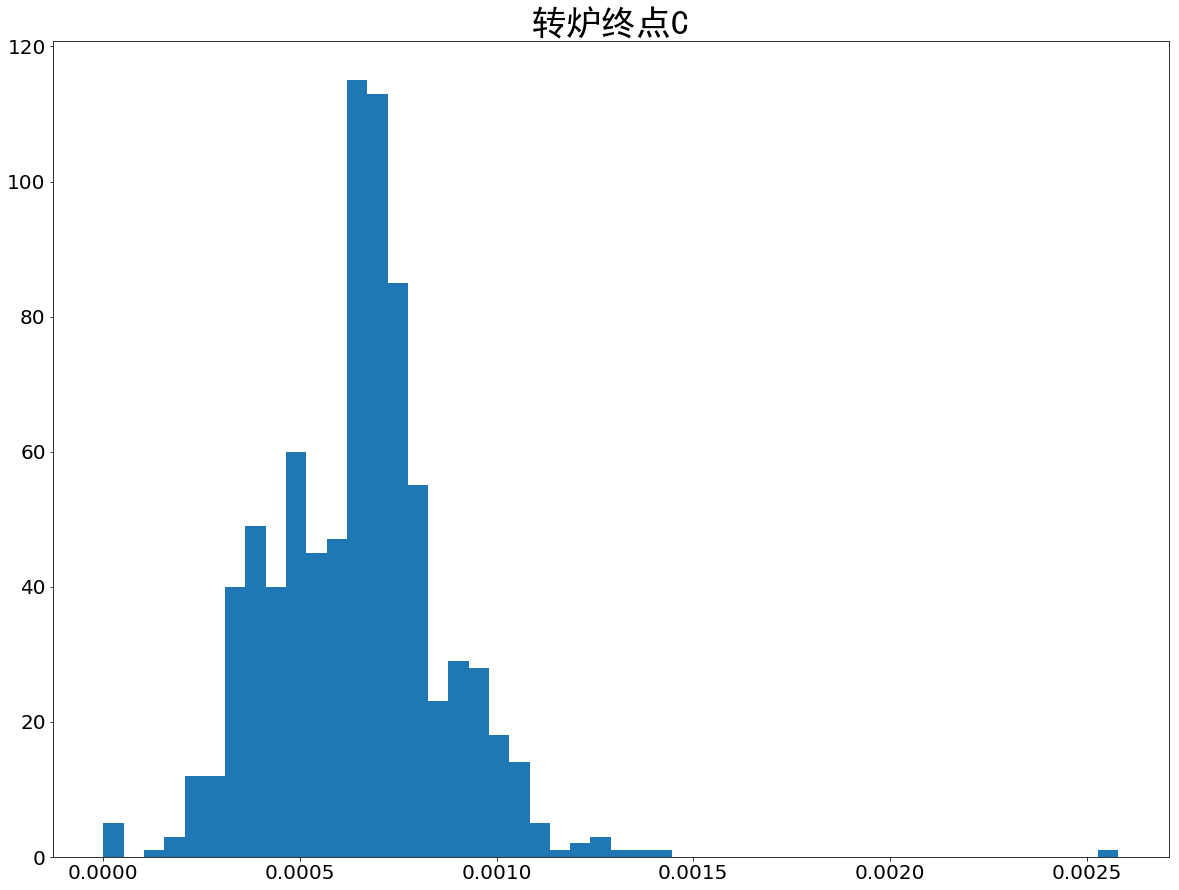
\includegraphics[width=0.45\textwidth]{fig/hist.png}
	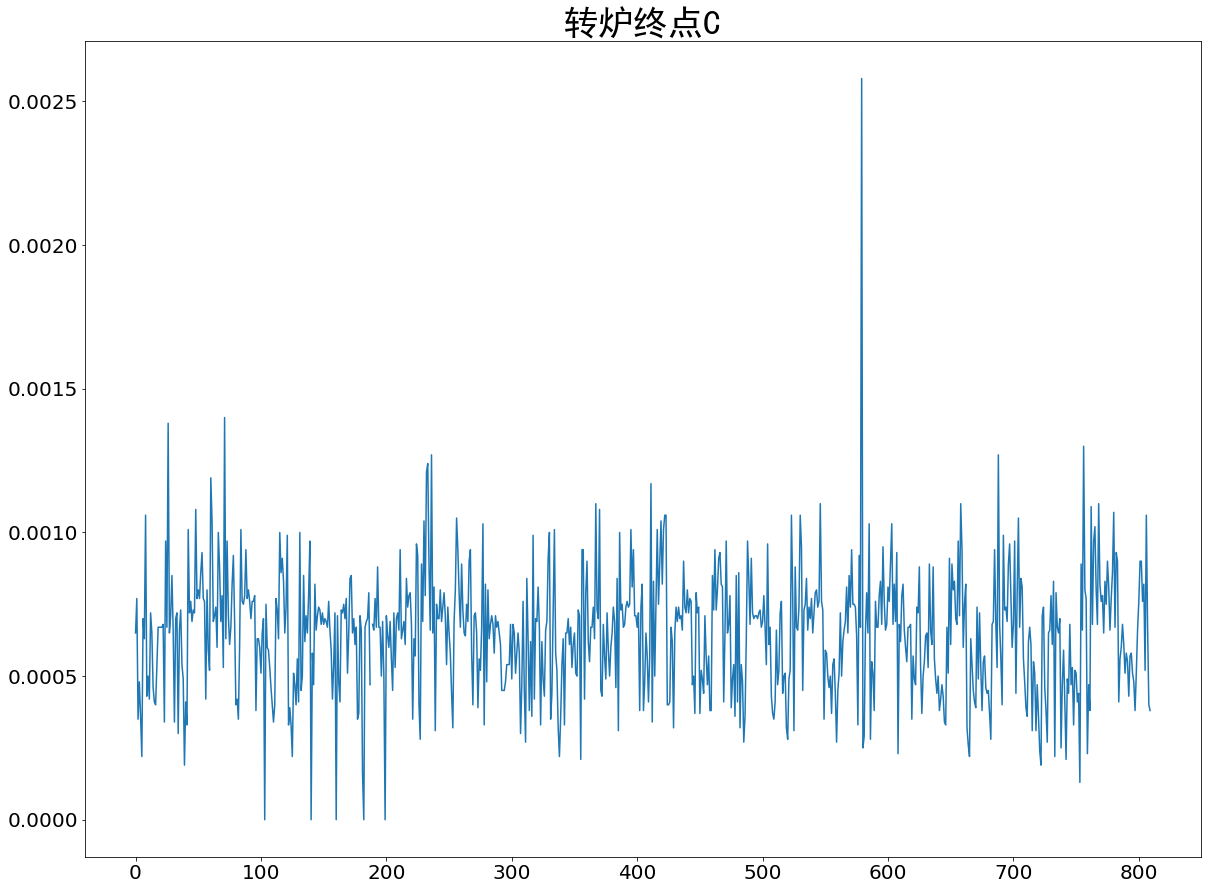
\includegraphics[width=0.45\textwidth]{fig/index.png}
	\caption{转炉终点C的数据分布\label{fig:prev}}
\end{figure}
\subsubsection{历史收得率的计算}
由题目可得,合金历史收得率的计算公式为:
\begin{equation} \label{eq:eps1}
    H_i=\frac{M(Out_i-Beg_i)}{T_i}\times 100\%
\end{equation}
  其中,$T_i$为添加配料中元素i的总质量,计算方式为$T_i=C_{i}^{T}X$,$X$为加入配料的质量构成的向量,$C_i$为每种配料对应元素i的含量。
$Beg_i$、$Out_i$分别为脱氧合金化前后钢水中元素i的含量。计算得到的历史收得率见附录。

\subsubsection{使用相关系数进行影响因素分析}
相关系数(Correlation coefficient)是反应变量之间关系密切程度的统计指标,相关系数的取值区间在1到-1之间。1表示两个变量完全线性相关,-1表示两个变量完全负相关,0表示两个变量不相关。数据越趋近于0表示相关关系越弱。公式\ref{eq:eps2}是相关系数的计算公式:
\begin{equation} \label{eq:eps2}
    r_{xy}=S_{xy}/(S_xS_y )
\end{equation}

其中$r_{xy}$ 表示样本相关系数,$S_{xy}$ 表示样本协方差,$S_x$ 表示$x$的样本标准差,$S_y$  表示$y$的样本标准差。下面分别是$S_{xy}$协方差和$S_x$和$S_y$标准差的计算公式。由于是样本协方差和样本标准差,因此分母使用的是$n-1$。
\[S_{xy}=\frac{\sum{i=1}^n(X_i-\overline{X})(Y_i-\overline{Y})}{n-1}\]
\[S_x=\sqrt{\frac{(X_i-\overline{X})^2}{n-1}}\]
\[S_y=\sqrt{\frac{(Y_i-\overline{Y})^2}{n-1}}\]

\par 我们分别计算了脱氧合金化过程中与C、Mn两种元素相关的变量与该元素收得率之间的相关系数,并保留了相关系数绝对值大于0.1的影
响因素,C、Mn相关系数见表\ref{tb:tbs1}、\ref{tb:tbs2}:
\begin{table}[htbp]
	\centering
	\begin{tabu}{l l}
		\tabucline[1.5pt]{-}
		影响因素 & C收得率\\
		\tabucline[1.5pt]{-}
		转炉终点C & -0.2888\\
		钢水净重 & 0.5026\\
		低铝硅铁 &0.4112\\
		石油焦增碳剂 & -0.2685\\
		\tabucline[1.5pt]{-}
	\end{tabu}
	\caption{C收得率与主要影响因素的相关系数\label{tb:tbs1}}
\end{table}
\begin{table}[htbp]
	\centering
	\begin{tabu}{l l}
		\\
		\tabucline[1.5pt]{-}
		影响因素 & Mn收得率\\
		\tabucline[1.5pt]{-}
		碳化硅(55\%) &-0.2163\\
		钒铁(FeV50-B).1 & -0.1861\\
		钒氮合金(进口) & 0.2486\\
		低铝硅铁 &	0.9407\\
		钢水净重 &	0.9440\\
		\tabucline[1.5pt]{-}
	\end{tabu}
	\caption{Mn收得率与主要影响因素的相关系数\label{tb:tbs2}}
\end{table}
\par 根据表\ref{tb:tbs1},C元素历史收得率的影响因素主要为C元素的转炉终点含量(脱氧合金化之前钢水中相应元素含量)、钢水净重、低铝硅铁、石油焦增碳剂。钢水净重与低铝硅铁于C元素的历史收得率呈正相关,钢水净重的影响表明钢水质量增加可以吸收更多的合金元素,转炉终点C和石油焦增碳剂对C元素历史收得率均有不同程度的负向响,表明加入过量的C化合物将导致C的收得率降低。根据表\ref{tb:tbs2},钢水净重、低硅铝铁和钒氮合金总体对Mn收得率有正向的影响,碳化硅和钒铁(FeV50-B)的加入更有可能使Mn收得率减小。
\begin{table}[htbp]
	\centering
	\begin{tabu}{l l |l l}
		\tabucline[1.5pt]{-}
		影响因素 & 回归系数 & 影响因素 & 回归系数\\
		\tabucline[1.5pt]{-}
		转炉终点温度  &  -0.0429 &  硅钙碳脱氧剂  &  -0.0158\\
		转炉终点C  &  -0.7986  &  转炉终点S  &  0.0012\\
		钢水净重  &  0.1989  &  氮化钒铁FeV55N11-A  &  -0.0468\\
		碳化硅(55\%)  &  -0.3568  &  钒氮合金(进口)  &  -0.0743\\
		钒铁(FeV50-A)  &  -0.0311  &  钒铁(FeV50-B)  &  -0.0\\
		钒铁(FeV50-B).1  &  -0.0276  &  硅铝钙  &  0.047\\
		硅铝合金FeAl30Si25  &  0.0545  &  硅铝锰合金球  &  0.0\\
		硅锰面(硅锰渣)  &  -0.0277  &  硅铁(合格块)  &  -0.0379\\
		硅铁FeSi75-B  &  -0.0449  &  石油焦增碳剂  &  -1.1481\\
		锰硅合金FeMn64Si27(合格块)  &  -0.1487  &  锰硅合金FeMn68Si18(合格块)  &  -0.2989\\
		\tabucline[1.5pt]{-}
	\end{tabu}
	\caption{C收得率线性回归模型对应系数\label{tb:tbs3}}
\end{table}

\subsubsection{使用线性回归进行影响因素分析}
\par 为了定量判断影响因素,首先进行数据的归一化处理,进而构建线性模型,从而可以通过模型的参数确定各影响因素及其影响程度。构建如式\ref{eq:esp3}线性模型:
\begin{equation}\label{eq:esp3}
	Y=\sum_{i=1}^na_iX_i+\varepsilon , \quad i=1,2,3,\ldots ,n
\end{equation}
其中$Y$为元素收得率,$X$为与该元素有关的影响因素,$a$为回归系数,表明该影响因素对元素收得率的影响程度,$n$为可能的影响因素数目,即加入合金配料的种类数,$\varepsilon$为偏差。

\par 对C收得率进行线性回归拟合,得到系数矩阵$[a_i]$及其对应变量如表\ref{tb:tbs3}。由于影响因素的变量数据经过了归一化,表中的回归系数大小可以定量的描述各个因素对C收得率的相对影响,钢水净重对元素收得率影响程度最大,且为较强的正相关关系,其次为C元素的转炉终点,二者具有较强的负相关关系;则更加石油焦增碳剂、锰硅合金、碳化硅(55\%)等的含量则会明显降低C元素的收得率,而增加硅铝钙的含量则会提高收得率。



\subsection{问题二的解答}
\subsubsection{问题二的分析}
\par 在问题1的基础上,本团队对预测模型进行了两点改进,第一,将变量中的缺失值用均值替代,一方面C、Mn元素的初始含量较低,对反应收得率影响较小,另一方面。第二,构建多种非线性模型改善算法,例如:决策树回归、SVM、贝叶斯、集成、多项式回归等,提高预测收得率准确性。

\subsubsection{数据预处理}
\begin{enumerate}[(a)]
\setlength{\itemindent}{2em}    %标签缩进量
\item 对数据进行离群值的去除处理,仅保留$[\mu-3\sigma,\mu-3\sigma]$范围内的数据,根据正态分布3σ原则,该范围理论上包括99.73\%的原始数据。
\item 对于样本缺失值较多的部分进行均值替代,一方面能够简化计算,另一方面能够提高分析结果的准确性与有效性。
\item 为方便后续数据的处理,对样本进行归一化处理。
\end{enumerate}

\subsubsection{模型的建立与求解}
\textbf{虚位以待}
\subsubsection{误差分析}
\textbf{虚位以待}

\subsection{问题三的解答}
\subsubsection{问题三的分析}
\par 本题涉及到目标函数最优化的问题,利用第二问的多项式预测模型对连铸合金的元素含量进行预测,进而根据题目所给HRB400B型号合金钢的元素含量标准建立线性约束。对于生产成本最低的最优合金配料方案问题,由于仅需要优化配料的成本,因此将未知的转炉终点元素含量以及转炉终点温度、钢水质量等无关变量全部使用均值替代,最终建立价格目标函数求解满足条件的最优方案。

\subsubsection{数据预处理}
\begin{enumerate}[(a)]
\setlength{\itemindent}{2em}    %标签缩进量
\item 离群值的处理。
\item 与第二问相同,缺失值用均值代替或丢弃。
\item 将不是配料的变量用均值进行替代,使其成为常量,为建立价格目标函数做准备。
\end{enumerate}

\subsubsection{模型的建立与求解}
为了简化模型的计算,我们选取线性模型进行C、Mn元素的收得率预测,并且为了保证预测结果处于HRB400B型合金钢元素国家标准含量区间内的条件下,建立如下约束条件:

基于上述条件,构建价格目标函数:
Price=AX
利用软件进行全局优化的求解,结果如下:



\section{模型的检验}
\section{进一步讨论}
\section{模型的优缺点}

\begin{thebibliography}{1}
\bibitem{1} 全国大学生数学建模竞赛组委会, 2004 高教社杯全国大学生数学建模竞赛论文格式规范, 2004
\bibitem{2} 全国大学生数学建模竞赛组委会, 2013 高教社杯全国大学生数学建模竞赛论文格式规范, 2013
\end{thebibliography}

\end{document}
